% REV00 Tue 04 May 2021 13:55:16 WIB
% START Tue 04 May 2021 13:55:16 WIB

\chapter{MR AND MRS BOFFIN IN CONSULTATION}

Betaking himself straight homeward, Mr Boffin, without further let or
hindrance, arrived at the Bower, and gave Mrs Boffin (in a walking dress
of black velvet and feathers, like a mourning coach-horse) an account of
all he had said and done since breakfast.

‘This brings us round, my dear,’ he then pursued, ‘to the question
we left unfinished: namely, whether there’s to be any new go-in for
Fashion.’

‘Now, I’ll tell you what I want, Noddy,’ said Mrs Boffin, smoothing her
dress with an air of immense enjoyment, ‘I want Society.’

‘Fashionable Society, my dear?’

‘Yes!’ cried Mrs Boffin, laughing with the glee of a child. ‘Yes! It’s
no good my being kept here like Wax-Work; is it now?’

‘People have to pay to see Wax-Work, my dear,’ returned her husband,
‘whereas (though you’d be cheap at the same money) the neighbours is
welcome to see YOU for nothing.’

‘But it don’t answer,’ said the cheerful Mrs Boffin. ‘When we worked
like the neighbours, we suited one another. Now we have left work off;
we have left off suiting one another.’

‘What, do you think of beginning work again?’ Mr Boffin hinted.

‘Out of the question! We have come into a great fortune, and we must do
what’s right by our fortune; we must act up to it.’

Mr Boffin, who had a deep respect for his wife’s intuitive wisdom,
replied, though rather pensively: ‘I suppose we must.’

‘It’s never been acted up to yet, and, consequently, no good has come of
it,’ said Mrs Boffin.

‘True, to the present time,’ Mr Boffin assented, with his former
pensiveness, as he took his seat upon his settle. ‘I hope good may be
coming of it in the future time. Towards which, what’s your views, old
lady?’

Mrs Boffin, a smiling creature, broad of figure and simple of nature,
with her hands folded in her lap, and with buxom creases in her throat,
proceeded to expound her views.

‘I say, a good house in a good neighbourhood, good things about us,
good living, and good society. I say, live like our means, without
extravagance, and be happy.’

‘Yes. I say be happy, too,’ assented the still pensive Mr Boffin.
‘Lor-a-mussy!’ exclaimed Mrs Boffin, laughing and clapping her hands,
and gaily rocking herself to and fro, ‘when I think of me in a light
yellow chariot and pair, with silver boxes to the wheels--’

‘Oh! you was thinking of that, was you, my dear?’

‘Yes!’ cried the delighted creature. ‘And with a footman up behind, with
a bar across, to keep his legs from being poled! And with a coachman
up in front, sinking down into a seat big enough for three of him, all
covered with upholstery in green and white! And with two bay horses
tossing their heads and stepping higher than they trot long-ways! And
with you and me leaning back inside, as grand as ninepence! Oh-h-h-h My!
Ha ha ha ha ha!’

Mrs Boffin clapped her hands again, rocked herself again, beat her feet
upon the floor, and wiped the tears of laughter from her eyes.

‘And what, my old lady,’ inquired Mr Boffin, when he also had
sympathetically laughed: ‘what’s your views on the subject of the
Bower?’

‘Shut it up. Don’t part with it, but put somebody in it, to keep it.’

‘Any other views?’

‘Noddy,’ said Mrs Boffin, coming from her fashionable sofa to his side
on the plain settle, and hooking her comfortable arm through his,
‘Next I think--and I really have been thinking early and late--of the
disappointed girl; her that was so cruelly disappointed, you know, both
of her husband and his riches. Don’t you think we might do something for
her? Have her to live with us? Or something of that sort?’

‘Ne-ver once thought of the way of doing it!’ cried Mr Boffin, smiting
the table in his admiration. ‘What a thinking steam-ingein this old lady
is. And she don’t know how she does it. Neither does the ingein!’

Mrs Boffin pulled his nearest ear, in acknowledgment of this piece of
philosophy, and then said, gradually toning down to a motherly strain:
‘Last, and not least, I have taken a fancy. You remember dear little
John Harmon, before he went to school? Over yonder across the yard, at
our fire? Now that he is past all benefit of the money, and it’s come to
us, I should like to find some orphan child, and take the boy and adopt
him and give him John’s name, and provide for him. Somehow, it would
make me easier, I fancy. Say it’s only a whim--’

‘But I don’t say so,’ interposed her husband.

‘No, but deary, if you did--’

‘I should be a Beast if I did,’ her husband interposed again.

‘That’s as much as to say you agree? Good and kind of you, and like you,
deary! And don’t you begin to find it pleasant now,’ said Mrs Boffin,
once more radiant in her comely way from head to foot, and once more
smoothing her dress with immense enjoyment, ‘don’t you begin to find
it pleasant already, to think that a child will be made brighter, and
better, and happier, because of that poor sad child that day? And isn’t
it pleasant to know that the good will be done with the poor sad child’s
own money?’

‘Yes; and it’s pleasant to know that you are Mrs Boffin,’ said her
husband, ‘and it’s been a pleasant thing to know this many and many a
year!’ It was ruin to Mrs Boffin’s aspirations, but, having so spoken,
they sat side by side, a hopelessly Unfashionable pair.

These two ignorant and unpolished people had guided themselves so far on
in their journey of life, by a religious sense of duty and desire to do
right. Ten thousand weaknesses and absurdities might have been detected
in the breasts of both; ten thousand vanities additional, possibly, in
the breast of the woman. But the hard wrathful and sordid nature that
had wrung as much work out of them as could be got in their best days,
for as little money as could be paid to hurry on their worst, had never
been so warped but that it knew their moral straightness and respected
it. In its own despite, in a constant conflict with itself and them, it
had done so. And this is the eternal law. For, Evil often stops short at
itself and dies with the doer of it; but Good, never.

Through his most inveterate purposes, the dead Jailer of Harmony Jail
had known these two faithful servants to be honest and true. While he
raged at them and reviled them for opposing him with the speech of the
honest and true, it had scratched his stony heart, and he had perceived
the powerlessness of all his wealth to buy them if he had addressed
himself to the attempt. So, even while he was their griping taskmaster
and never gave them a good word, he had written their names down in his
will. So, even while it was his daily declaration that he mistrusted all
mankind--and sorely indeed he did mistrust all who bore any resemblance
to himself--he was as certain that these two people, surviving him,
would be trustworthy in all things from the greatest to the least, as he
was that he must surely die.

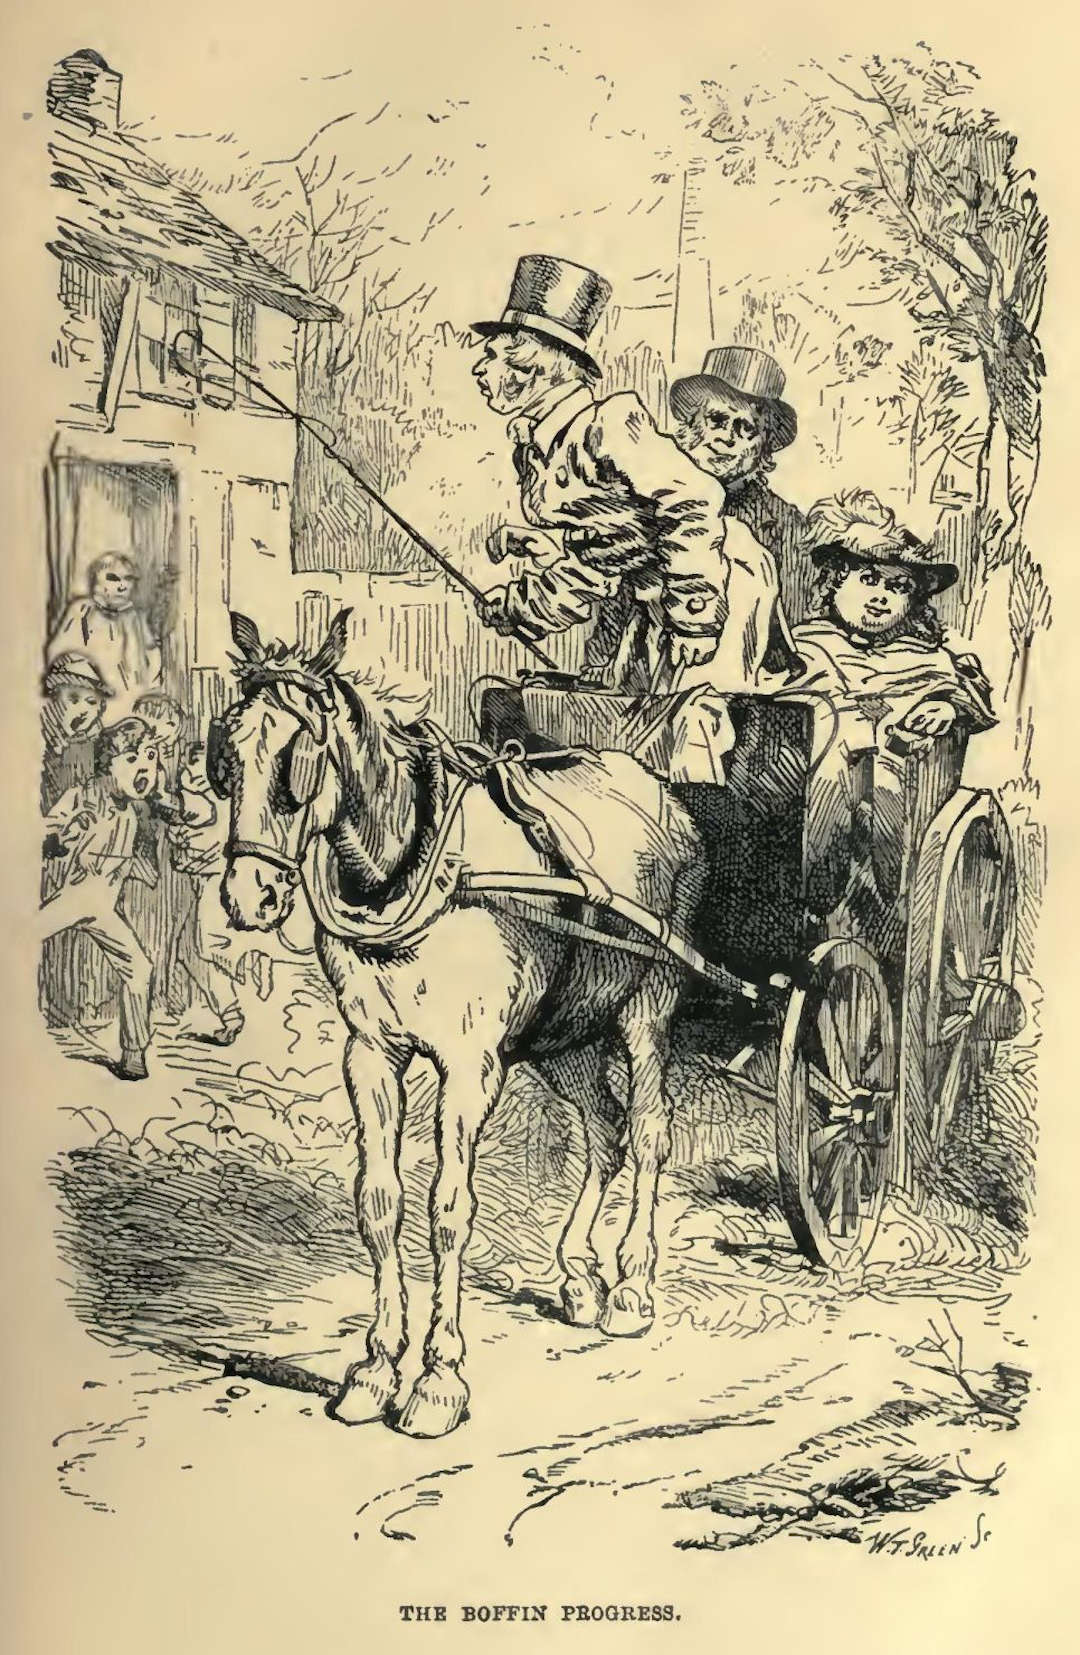
\includegraphics[scale=2.3]{01-09-01}

Mr and Mrs Boffin, sitting side by side, with Fashion withdrawn to an
immeasurable distance, fell to discussing how they could best find their
orphan. Mrs Boffin suggested advertisement in the newspapers, requesting
orphans answering annexed description to apply at the Bower on a certain
day; but Mr Boffin wisely apprehending obstruction of the neighbouring
thoroughfares by orphan swarms, this course was negatived. Mrs Boffin
next suggested application to their clergyman for a likely orphan. Mr
Boffin thinking better of this scheme, they resolved to call upon the
reverend gentleman at once, and to take the same opportunity of making
acquaintance with Miss Bella Wilfer. In order that these visits might be
visits of state, Mrs Boffin’s equipage was ordered out.

This consisted of a long hammer-headed old horse, formerly used in the
business, attached to a four-wheeled chaise of the same period, which
had long been exclusively used by the Harmony Jail poultry as the
favourite laying-place of several discreet hens. An unwonted application
of corn to the horse, and of paint and varnish to the carriage, when
both fell in as a part of the Boffin legacy, had made what Mr Boffin
considered a neat turn-out of the whole; and a driver being added, in
the person of a long hammer-headed young man who was a very good match
for the horse, left nothing to be desired. He, too, had been formerly
used in the business, but was now entombed by an honest jobbing tailor
of the district in a perfect Sepulchre of coat and gaiters, sealed with
ponderous buttons.

Behind this domestic, Mr and Mrs Boffin took their seats in the back
compartment of the vehicle: which was sufficiently commodious, but had
an undignified and alarming tendency, in getting over a rough crossing,
to hiccup itself away from the front compartment. On their being
descried emerging from the gates of the Bower, the neighbourhood turned
out at door and window to salute the Boffins. Among those who were ever
and again left behind, staring after the equipage, were many youthful
spirits, who hailed it in stentorian tones with such congratulations as
‘Nod-dy Bof-fin!’ ‘Bof-fin’s mon-ey!’ ‘Down with the dust, Bof-fin!’ and
other similar compliments. These, the hammer-headed young man took in
such ill part that he often impaired the majesty of the progress by
pulling up short, and making as though he would alight to exterminate
the offenders; a purpose from which he only allowed himself to be
dissuaded after long and lively arguments with his employers.

At length the Bower district was left behind, and the peaceful dwelling
of the Reverend Frank Milvey was gained. The Reverend Frank Milvey’s
abode was a very modest abode, because his income was a very modest
income. He was officially accessible to every blundering old woman who
had incoherence to bestow upon him, and readily received the Boffins.
He was quite a young man, expensively educated and wretchedly paid, with
quite a young wife and half a dozen quite young children. He was under
the necessity of teaching and translating from the classics, to eke out
his scanty means, yet was generally expected to have more time to spare
than the idlest person in the parish, and more money than the richest.
He accepted the needless inequalities and inconsistencies of his life,
with a kind of conventional submission that was almost slavish; and any
daring layman who would have adjusted such burdens as his, more decently
and graciously, would have had small help from him.

With a ready patient face and manner, and yet with a latent smile that
showed a quick enough observation of Mrs Boffin’s dress, Mr Milvey, in
his little book-room--charged with sounds and cries as though the six
children above were coming down through the ceiling, and the roasting
leg of mutton below were coming up through the floor--listened to Mrs
Boffin’s statement of her want of an orphan.

‘I think,’ said Mr Milvey, ‘that you have never had a child of your own,
Mr and Mrs Boffin?’

Never.

‘But, like the Kings and Queens in the Fairy Tales, I suppose you have
wished for one?’

In a general way, yes.

Mr Milvey smiled again, as he remarked to himself ‘Those kings and
queens were always wishing for children.’ It occurring to him, perhaps,
that if they had been Curates, their wishes might have tended in the
opposite direction.

‘I think,’ he pursued, ‘we had better take Mrs Milvey into our Council.
She is indispensable to me. If you please, I’ll call her.’

So, Mr Milvey called, ‘Margaretta, my dear!’ and Mrs Milvey came down.
A pretty, bright little woman, something worn by anxiety, who had
repressed many pretty tastes and bright fancies, and substituted in
their stead, schools, soup, flannel, coals, and all the week-day cares
and Sunday coughs of a large population, young and old. As gallantly had
Mr Milvey repressed much in himself that naturally belonged to his old
studies and old fellow-students, and taken up among the poor and their
children with the hard crumbs of life.

‘Mr and Mrs Boffin, my dear, whose good fortune you have heard of.’

Mrs Milvey, with the most unaffected grace in the world, congratulated
them, and was glad to see them. Yet her engaging face, being an open as
well as a perceptive one, was not without her husband’s latent smile.

‘Mrs Boffin wishes to adopt a little boy, my dear.’

Mrs Milvey, looking rather alarmed, her husband added:

‘An orphan, my dear.’

‘Oh!’ said Mrs Milvey, reassured for her own little boys.

‘And I was thinking, Margaretta, that perhaps old Mrs Goody’s grandchild
might answer the purpose.

‘Oh my DEAR Frank! I DON’T think that would do!’

‘No?’

‘Oh NO!’

The smiling Mrs Boffin, feeling it incumbent on her to take part in the
conversation, and being charmed with the emphatic little wife and her
ready interest, here offered her acknowledgments and inquired what there
was against him?

‘I DON’T think,’ said Mrs Milvey, glancing at the Reverend Frank, ‘--and
I believe my husband will agree with me when he considers it again--that
you could possibly keep that orphan clean from snuff. Because his
grandmother takes so MANY ounces, and drops it over him.’

‘But he would not be living with his grandmother then, Margaretta,’ said
Mr Milvey.

‘No, Frank, but it would be impossible to keep her from Mrs Boffin’s
house; and the MORE there was to eat and drink there, the oftener she
would go. And she IS an inconvenient woman. I HOPE it’s not uncharitable
to remember that last Christmas Eve she drank eleven cups of tea, and
grumbled all the time. And she is NOT a grateful woman, Frank. You
recollect her addressing a crowd outside this house, about her wrongs,
when, one night after we had gone to bed, she brought back the petticoat
of new flannel that had been given her, because it was too short.’

‘That’s true,’ said Mr Milvey. ‘I don’t think that would do. Would
little Harrison--’

‘Oh, FRANK!’ remonstrated his emphatic wife.

‘He has no grandmother, my dear.’

‘No, but I DON’T think Mrs Boffin would like an orphan who squints so
MUCH.’

‘That’s true again,’ said Mr Milvey, becoming haggard with perplexity.
‘If a little girl would do--’

‘But, my DEAR Frank, Mrs Boffin wants a boy.’

‘That’s true again,’ said Mr Milvey. ‘Tom Bocker is a nice boy’
(thoughtfully).

‘But I DOUBT, Frank,’ Mrs Milvey hinted, after a little hesitation, ‘if
Mrs Boffin wants an orphan QUITE nineteen, who drives a cart and waters
the roads.’

Mr Milvey referred the point to Mrs Boffin in a look; on that smiling
lady’s shaking her black velvet bonnet and bows, he remarked, in lower
spirits, ‘that’s true again.’

‘I am sure,’ said Mrs Boffin, concerned at giving so much trouble, ‘that
if I had known you would have taken so much pains, sir--and you too, ma’
am--I don’t think I would have come.’

‘PRAY don’t say that!’ urged Mrs Milvey.

‘No, don’t say that,’ assented Mr Milvey, ‘because we are so much
obliged to you for giving us the preference.’ Which Mrs Milvey
confirmed; and really the kind, conscientious couple spoke, as if they
kept some profitable orphan warehouse and were personally patronized.
‘But it is a responsible trust,’ added Mr Milvey, ‘and difficult to
discharge. At the same time, we are naturally very unwilling to lose the
chance you so kindly give us, and if you could afford us a day or two
to look about us,--you know, Margaretta, we might carefully examine the
workhouse, and the Infant School, and your District.’

‘To be SURE!’ said the emphatic little wife.

‘We have orphans, I know,’ pursued Mr Milvey, quite with the air as if
he might have added, ‘in stock,’ and quite as anxiously as if there were
great competition in the business and he were afraid of losing an order,
‘over at the clay-pits; but they are employed by relations or friends,
and I am afraid it would come at last to a transaction in the way of
barter. And even if you exchanged blankets for the child--or books
and firing--it would be impossible to prevent their being turned into
liquor.’

Accordingly, it was resolved that Mr and Mrs Milvey should search for
an orphan likely to suit, and as free as possible from the foregoing
objections, and should communicate again with Mrs Boffin. Then, Mr
Boffin took the liberty of mentioning to Mr Milvey that if Mr Milvey
would do him the kindness to be perpetually his banker to the extent
of ‘a twenty-pound note or so,’ to be expended without any reference
to him, he would be heartily obliged. At this, both Mr Milvey and Mrs
Milvey were quite as much pleased as if they had no wants of their own,
but only knew what poverty was, in the persons of other people; and
so the interview terminated with satisfaction and good opinion on all
sides.

‘Now, old lady,’ said Mr Boffin, as they resumed their seats behind the
hammer-headed horse and man: ‘having made a very agreeable visit there,
we’ll try Wilfer’s.’

It appeared, on their drawing up at the family gate, that to try
Wilfer’s was a thing more easily projected than done, on account of the
extreme difficulty of getting into that establishment; three pulls
at the bell producing no external result; though each was attended
by audible sounds of scampering and rushing within. At the fourth
tug--vindictively administered by the hammer-headed young man--Miss
Lavinia appeared, emerging from the house in an accidental manner, with
a bonnet and parasol, as designing to take a contemplative walk. The
young lady was astonished to find visitors at the gate, and expressed
her feelings in appropriate action.

‘Here’s Mr and Mrs Boffin!’ growled the hammer-headed young man through
the bars of the gate, and at the same time shaking it, as if he were on
view in a Menagerie; ‘they’ve been here half an hour.’

‘Who did you say?’ asked Miss Lavinia.

‘Mr and Mrs BOFFIN’ returned the young man, rising into a roar.

Miss Lavinia tripped up the steps to the house-door, tripped down the
steps with the key, tripped across the little garden, and opened the
gate. ‘Please to walk in,’ said Miss Lavinia, haughtily. ‘Our servant is
out.’

Mr and Mrs Boffin complying, and pausing in the little hall until Miss
Lavinia came up to show them where to go next, perceived three pairs of
listening legs upon the stairs above. Mrs Wilfer’s legs, Miss Bella’s
legs, Mr George Sampson’s legs.

‘Mr and Mrs Boffin, I think?’ said Lavinia, in a warning voice. Strained
attention on the part of Mrs Wilfer’s legs, of Miss Bella’s legs, of Mr
George Sampson’s legs.

‘Yes, Miss.’

‘If you’ll step this way--down these stairs--I’ll let Ma know.’
Excited flight of Mrs Wilfer’s legs, of Miss Bella’s legs, of Mr George
Sampson’s legs.

After waiting some quarter of an hour alone in the family sitting-room,
which presented traces of having been so hastily arranged after a meal,
that one might have doubted whether it was made tidy for visitors,
or cleared for blindman’s buff, Mr and Mrs Boffin became aware of the
entrance of Mrs Wilfer, majestically faint, and with a condescending
stitch in her side: which was her company manner.

‘Pardon me,’ said Mrs Wilfer, after the first salutations, and as soon
as she had adjusted the handkerchief under her chin, and waved her
gloved hands, ‘to what am I indebted for this honour?’

‘To make short of it, ma’am,’ returned Mr Boffin, ‘perhaps you may be
acquainted with the names of me and Mrs Boffin, as having come into a
certain property.’

‘I have heard, sir,’ returned Mrs Wilfer, with a dignified bend of her
head, ‘of such being the case.’

‘And I dare say, ma’am,’ pursued Mr Boffin, while Mrs Boffin added
confirmatory nods and smiles, ‘you are not very much inclined to take
kindly to us?’

‘Pardon me,’ said Mrs Wilfer. ‘’Twere unjust to visit upon Mr and Mrs
Boffin, a calamity which was doubtless a dispensation.’ These words
were rendered the more effective by a serenely heroic expression of
suffering.

‘That’s fairly meant, I am sure,’ remarked the honest Mr Boffin; ‘Mrs
Boffin and me, ma’am, are plain people, and we don’t want to pretend
to anything, nor yet to go round and round at anything because there’s
always a straight way to everything. Consequently, we make this call
to say, that we shall be glad to have the honour and pleasure of your
daughter’s acquaintance, and that we shall be rejoiced if your daughter
will come to consider our house in the light of her home equally with
this. In short, we want to cheer your daughter, and to give her
the opportunity of sharing such pleasures as we are a going to take
ourselves. We want to brisk her up, and brisk her about, and give her a
change.’

‘That’s it!’ said the open-hearted Mrs Boffin. ‘Lor! Let’s be
comfortable.’

Mrs Wilfer bent her head in a distant manner to her lady visitor, and
with majestic monotony replied to the gentleman:

‘Pardon me. I have several daughters. Which of my daughters am I to
understand is thus favoured by the kind intentions of Mr Boffin and his
lady?’

‘Don’t you see?’ the ever-smiling Mrs Boffin put in. ‘Naturally, Miss
Bella, you know.’

‘Oh-h!’ said Mrs Wilfer, with a severely unconvinced look. ‘My daughter
Bella is accessible and shall speak for herself.’ Then opening the door
a little way, simultaneously with a sound of scuttling outside it,
the good lady made the proclamation, ‘Send Miss Bella to me!’ which
proclamation, though grandly formal, and one might almost say heraldic,
to hear, was in fact enunciated with her maternal eyes reproachfully
glaring on that young lady in the flesh--and in so much of it that she
was retiring with difficulty into the small closet under the stairs,
apprehensive of the emergence of Mr and Mrs Boffin.

‘The avocations of R. W., my husband,’ Mrs Wilfer explained, on resuming
her seat, ‘keep him fully engaged in the City at this time of the day,
or he would have had the honour of participating in your reception
beneath our humble roof.’

‘Very pleasant premises!’ said Mr Boffin, cheerfully.

‘Pardon me, sir,’ returned Mrs Wilfer, correcting him, ‘it is the abode
of conscious though independent Poverty.’

Finding it rather difficult to pursue the conversation down this road,
Mr and Mrs Boffin sat staring at mid-air, and Mrs Wilfer sat silently
giving them to understand that every breath she drew required to be
drawn with a self-denial rarely paralleled in history, until Miss Bella
appeared: whom Mrs Wilfer presented, and to whom she explained the
purpose of the visitors.

‘I am much obliged to you, I am sure,’ said Miss Bella, coldly shaking
her curls, ‘but I doubt if I have the inclination to go out at all.’

‘Bella!’ Mrs Wilfer admonished her; ‘Bella, you must conquer this.’

‘Yes, do what your Ma says, and conquer it, my dear,’ urged Mrs Boffin,
‘because we shall be so glad to have you, and because you are much too
pretty to keep yourself shut up.’ With that, the pleasant creature gave
her a kiss, and patted her on her dimpled shoulders; Mrs Wilfer sitting
stiffly by, like a functionary presiding over an interview previous to
an execution.

‘We are going to move into a nice house,’ said Mrs Boffin, who was woman
enough to compromise Mr Boffin on that point, when he couldn’t very well
contest it; ‘and we are going to set up a nice carriage, and we’ll go
everywhere and see everything. And you mustn’t,’ seating Bella beside
her, and patting her hand, ‘you mustn’t feel a dislike to us to begin
with, because we couldn’t help it, you know, my dear.’

With the natural tendency of youth to yield to candour and sweet temper,
Miss Bella was so touched by the simplicity of this address that she
frankly returned Mrs Boffin’s kiss. Not at all to the satisfaction
of that good woman of the world, her mother, who sought to hold the
advantageous ground of obliging the Boffins instead of being obliged.

‘My youngest daughter, Lavinia,’ said Mrs Wilfer, glad to make a
diversion, as that young lady reappeared. ‘Mr George Sampson, a friend
of the family.’

The friend of the family was in that stage of tender passion which bound
him to regard everybody else as the foe of the family. He put the round
head of his cane in his mouth, like a stopper, when he sat down. As if
he felt himself full to the throat with affronting sentiments. And he
eyed the Boffins with implacable eyes.

‘If you like to bring your sister with you when you come to stay with
us,’ said Mrs Boffin, ‘of course we shall be glad. The better you please
yourself, Miss Bella, the better you’ll please us.’

‘Oh, my consent is of no consequence at all, I suppose?’ cried Miss
Lavinia.

‘Lavvy,’ said her sister, in a low voice, ‘have the goodness to be seen
and not heard.’

‘No, I won’t,’ replied the sharp Lavinia. ‘I’m not a child, to be taken
notice of by strangers.’

‘You ARE a child.’

‘I’m not a child, and I won’t be taken notice of. “Bring your sister,”
 indeed!’

‘Lavinia!’ said Mrs Wilfer. ‘Hold! I will not allow you to utter in my
presence the absurd suspicion that any strangers--I care not what their
names--can patronize my child. Do you dare to suppose, you ridiculous
girl, that Mr and Mrs Boffin would enter these doors upon a patronizing
errand; or, if they did, would remain within them, only for one single
instant, while your mother had the strength yet remaining in her vital
frame to request them to depart? You little know your mother if you
presume to think so.’

‘It’s all very fine,’ Lavinia began to grumble, when Mrs Wilfer
repeated:

‘Hold! I will not allow this. Do you not know what is due to guests?
Do you not comprehend that in presuming to hint that this lady and
gentleman could have any idea of patronizing any member of your
family--I care not which--you accuse them of an impertinence little less
than insane?’

‘Never mind me and Mrs Boffin, ma’am,’ said Mr Boffin, smilingly: ‘we
don’t care.’

‘Pardon me, but I do,’ returned Mrs Wilfer.

Miss Lavinia laughed a short laugh as she muttered, ‘Yes, to be sure.’

‘And I require my audacious child,’ proceeded Mrs Wilfer, with a
withering look at her youngest, on whom it had not the slightest effect,
‘to please to be just to her sister Bella; to remember that her sister
Bella is much sought after; and that when her sister Bella accepts an
attention, she considers herself to be conferring qui-i-ite as much
honour,’--this with an indignant shiver,--‘as she receives.’

But, here Miss Bella repudiated, and said quietly, ‘I can speak for
myself; you know, ma. You needn’t bring ME in, please.’

‘And it’s all very well aiming at others through convenient me,’ said
the irrepressible Lavinia, spitefully; ‘but I should like to ask George
Sampson what he says to it.’

‘Mr Sampson,’ proclaimed Mrs Wilfer, seeing that young gentleman take
his stopper out, and so darkly fixing him with her eyes as that he put
it in again: ‘Mr Sampson, as a friend of this family and a frequenter of
this house, is, I am persuaded, far too well-bred to interpose on such
an invitation.’

This exaltation of the young gentleman moved the conscientious Mrs
Boffin to repentance for having done him an injustice in her mind, and
consequently to saying that she and Mr Boffin would at any time be glad
to see him; an attention which he handsomely acknowledged by replying,
with his stopper unremoved, ‘Much obliged to you, but I’m always
engaged, day and night.’

However, Bella compensating for all drawbacks by responding to the
advances of the Boffins in an engaging way, that easy pair were on the
whole well satisfied, and proposed to the said Bella that as soon as
they should be in a condition to receive her in a manner suitable to
their desires, Mrs Boffin should return with notice of the fact. This
arrangement Mrs Wilfer sanctioned with a stately inclination of her
head and wave of her gloves, as who should say, ‘Your demerits shall be
overlooked, and you shall be mercifully gratified, poor people.’

‘By-the-bye, ma’am,’ said Mr Boffin, turning back as he was going, ‘you
have a lodger?’

‘A gentleman,’ Mrs Wilfer answered, qualifying the low expression,
‘undoubtedly occupies our first floor.’

‘I may call him Our Mutual Friend,’ said Mr Boffin. ‘What sort of a
fellow IS Our Mutual Friend, now? Do you like him?’

‘Mr Rokesmith is very punctual, very quiet, a very eligible inmate.’

‘Because,’ Mr Boffin explained, ‘you must know that I’m not particularly
well acquainted with Our Mutual Friend, for I have only seen him once.
You give a good account of him. Is he at home?’

‘Mr Rokesmith is at home,’ said Mrs Wilfer; ‘indeed,’ pointing through
the window, ‘there he stands at the garden gate. Waiting for you,
perhaps?’

‘Perhaps so,’ replied Mr Boffin. ‘Saw me come in, maybe.’

Bella had closely attended to this short dialogue. Accompanying Mrs
Boffin to the gate, she as closely watched what followed.

‘How are you, sir, how are you?’ said Mr Boffin. ‘This is Mrs Boffin. Mr
Rokesmith, that I told you of; my dear.’

She gave him good day, and he bestirred himself and helped her to her
seat, and the like, with a ready hand.

‘Good-bye for the present, Miss Bella,’ said Mrs Boffin, calling out a
hearty parting. ‘We shall meet again soon! And then I hope I shall have
my little John Harmon to show you.’

Mr Rokesmith, who was at the wheel adjusting the skirts of her dress,
suddenly looked behind him, and around him, and then looked up at her,
with a face so pale that Mrs Boffin cried:

‘Gracious!’ And after a moment, ‘What’s the matter, sir?’

‘How can you show her the Dead?’ returned Mr Rokesmith.

‘It’s only an adopted child. One I have told her of. One I’m going to
give the name to!’

‘You took me by surprise,’ said Mr Rokesmith, ‘and it sounded like an
omen, that you should speak of showing the Dead to one so young and
blooming.’

Now, Bella suspected by this time that Mr Rokesmith admired her. Whether
the knowledge (for it was rather that than suspicion) caused her to
incline to him a little more, or a little less, than she had done at
first; whether it rendered her eager to find out more about him, because
she sought to establish reason for her distrust, or because she sought
to free him from it; was as yet dark to her own heart. But at most
times he occupied a great amount of her attention, and she had set her
attention closely on this incident.

That he knew it as well as she, she knew as well as he, when they were
left together standing on the path by the garden gate.

‘Those are worthy people, Miss Wilfer.’

‘Do you know them well?’ asked Bella.

He smiled, reproaching her, and she coloured, reproaching herself--both,
with the knowledge that she had meant to entrap him into an answer not
true--when he said ‘I know OF them.’

‘Truly, he told us he had seen you but once.’

‘Truly, I supposed he did.’

Bella was nervous now, and would have been glad to recall her question.

‘You thought it strange that, feeling much interested in you, I should
start at what sounded like a proposal to bring you into contact with the
murdered man who lies in his grave. I might have known--of course in a
moment should have known--that it could not have that meaning. But my
interest remains.’

Re-entering the family-room in a meditative state, Miss Bella was
received by the irrepressible Lavinia with:

‘There, Bella! At last I hope you have got your wishes realized--by your
Boffins. You’ll be rich enough now--with your Boffins. You can have as
much flirting as you like--at your Boffins. But you won’t take ME to
your Boffins, I can tell you--you and your Boffins too!’

‘If,’ quoth Mr George Sampson, moodily pulling his stopper out, ‘Miss
Bella’s Mr Boffin comes any more of his nonsense to ME, I only wish him
to understand, as betwixt man and man, that he does it at his per--’ and
was going to say peril; but Miss Lavinia, having no confidence in his
mental powers, and feeling his oration to have no definite application
to any circumstances, jerked his stopper in again, with a sharpness that
made his eyes water.

And now the worthy Mrs Wilfer, having used her youngest daughter as a
lay-figure for the edification of these Boffins, became bland to her,
and proceeded to develop her last instance of force of character,
which was still in reserve. This was, to illuminate the family with her
remarkable powers as a physiognomist; powers that terrified R. W. when
ever let loose, as being always fraught with gloom and evil which no
inferior prescience was aware of. And this Mrs Wilfer now did, be it
observed, in jealousy of these Boffins, in the very same moments when
she was already reflecting how she would flourish these very same
Boffins and the state they kept, over the heads of her Boffinless
friends.

‘Of their manners,’ said Mrs Wilfer, ‘I say nothing. Of their
appearance, I say nothing. Of the disinterestedness of their intentions
towards Bella, I say nothing. But the craft, the secrecy, the dark
deep underhanded plotting, written in Mrs Boffin’s countenance, make me
shudder.’

As an incontrovertible proof that those baleful attributes were all
there, Mrs Wilfer shuddered on the spot.


